\documentclass[a4paper,12pt]{article}
\usepackage[utf8]{inputenc}
\usepackage[french]{babel}
\usepackage[T1]{fontenc}
\usepackage[top=2cm,bottom=2cm,left=2cm,right=2cm]{geometry}
\usepackage{graphicx}
\usepackage{enumitem}
\usepackage{hyperref}
\usepackage{listings}
\usepackage{array}
\usepackage[ruled,vlined]{algorithm2e}
\usepackage{algpseudocode}
\usepackage{amsmath}
\usepackage{pgfplots}
\usepackage{tikz} 
\usepackage{caption}
\usepackage{subcaption}
\usepackage{float}

\title{Rapport Projet - Analyse des algorithmes de tri ABBA}
\author{Baptiste Borie, Benjamin Boutrois, Aboubacar Keita, Akram Zahry}
\date{Avril 2024}

\begin{document}
\maketitle
\begin{figure}[h]
\centering

\includegraphics[width=0.6\textwidth]{unilogo.png}
\end{figure}
\newpage
\tableofcontents
\newpage
\section{Introduction}
Après avoir défini les groupes nous avons longuement discutés entre nous sur le choix du sujet. Finalement notre choix s'est porté sur l'analyse d'algorithmes de tri. Notre but avec ce projet était de définir : quel est l'efficacité des algorithmes en fonction de la liste à trier (taille et type de désordre) ? 

Les algorithmes de tri constituent un élément fondamental de l'informatique, utilisés dans une variété d'applications pour organiser des données de manière efficace. Ce projet se concentre sur l'analyse comparative des performances des algorithmes de tri en fonction du niveau de désordre des données en entrée. Pour cela, nous avons mis en place un générateur de désordres maîtrisés sur les listes et avons implémenté une variété d'algorithmes de tri. Ce rapport présente nos résultats et analyses, offrant ainsi un aperçu des performances relatives de ces algorithmes dans des scénarios réalistes de traitement de données.


Nous avons décidé de nous répartir le sujet en 3 parties. Aboubacar et Akram se sont chargés d'implémenter autant d'algorithmes que possible. Benjamin avait pour rôle de réaliser des générateurs de désordre selon des critères définis enfin, l'objectif de Baptiste était de réaliser une visualisation claire des algorithmes et de leur tri ainsi que d'intégrer le modèle à la vue grâce à un contrôleur.

\section{Objectifs du Projet}

Ce projet a été conçu avec plusieurs objectifs clés visant à explorer et à analyser les performances des algorithmes de tri dans divers contextes. Les objectifs principaux comprenaient :

\begin{enumerate}
\item \textbf{Analyse comparative des performances} : L'objectif principal de ce projet était de réaliser une étude comparative approfondie des performances des algorithmes de tri. Cela impliquait de mesurer et de comparer le nombre de comparaisons, les accès aux données et les temps d'exécution pour une variété d'algorithmes de tri dans différentes situations.

\item \textbf{Étude de la sensibilité au désordre des données} : Nous avons cherché à évaluer comment les performances des algorithmes de tri étaient affectées par le niveau de désordre des données en entrée. En analysant cette sensibilité, nous voulions identifier les algorithmes les plus adaptés à des ensembles de données plus ou moins désordonnés.

\item \textbf{Développement d'outils de visualisation} : Un autre objectif était de créer des outils de visualisation permettant d'observer de manière intuitive l'exécution des algorithmes de tri. Ces visualisations devaient faciliter la compréhension du comportement de chaque algorithme et mettre en évidence les différences de performance entre eux.

\end{enumerate}

En atteignant ces objectifs, nous espérions fournir des résultats significatifs sur la sélection et l'utilisation d'algorithmes de tri dans des applications pratiques, tout en contribuant à l'enrichissement de la compréhension générale de ces techniques fondamentales en informatique.


\section{Modèle}
\subsection{Les tris implémenté}
Pour mener à bien notre étude comparative des algorithmes de tri, nous avons implémenté une variété de techniques de tri, chacune présentant des caractéristiques et des performances différentes. Voici une liste des algorithmes de tri que nous avons inclus dans notre étude : \\

\begin{itemize}

\item \textbf{BubbleSort} : Nous avons implémenté le classique algorithme de tri à bulles, qui consiste à parcourir répétitivement le tableau et à échanger les éléments adjacents s'ils sont dans le mauvais ordre. Cependant, sa complexité en temps est $O(n^2)$ dans le pire des cas, ce qui le rend peu performant pour de grandes listes. Néanmoins, il est facile à implémenter et peut être utilisé pour de petites quantités de données ou dans des cas où la performance n'est pas une priorité. L'algorithme s'arrête dès qu'aucun échange n'est effectué pendant un passage complet sur la liste, ce qui améliore sa performance dans certains cas. \\

\item \textbf{FusionSort} : Le tri fusion est un algorithme efficace qui utilise le principe de diviser pour régner. Il fonctionne en divisant récursivement la liste à trier en deux moitiés jusqu'à ce que chaque moitié ne contienne qu'un seul élément, puis fusionne ces moitiés de manière ordonnée pour obtenir la liste triée finale.
L'algorithme de tri fusion est apprécié pour sa stabilité, sa rapidité et son efficacité sur de grandes quantités de données. Sa complexité temporelle est O(n log n), ce qui en fait l'un des algorithmes de tri les plus rapides dans de nombreux situation.
La récursivité est au cœur de l'algorithme de tri fusion, par ce que la division répétée de la liste en sous-listes de plus en plus petites garantit que chaque sous-liste est triée avant la fusion, ce qui garantit que la liste finale sera également triée.
Bien que le tri fusion soit efficace pour de grandes quantités de données, mais  il peut être très gourmand en mémoire par rapport a d’autres types d’algo de tri à cause de la récursivité et aussi le fait de stocker temporairement des listes. Cependant, dans de nombreux cas, ses performances en termes de temps de calcul compensent largement cette exigence en mémoire.\\

\item \textbf{CombSort} : Cette méthode de tri améliore le tri à bulles.l fonctionne en comparant et en échangeant  les éléments avec un écart initial, qui diminue progressivement à chaque itération. Le code commence par initialiser l'écart à la taille de la liste, puis exécute une boucle jusqu'à ce que l'écart devienne 1 et aucun échange n'ait été effectué. À chaque itération, l'algorithme calcule le prochain écart en utilisant une formule spécifique, puis parcourt la liste en comparant les éléments distants de cet écart et en les échangeant s’il le faut nécessaire. \\

\item \textbf{InsertionSort} : Cet algorithme n’est efficace que pour trier de petites quantités de données ou des listes presque triées. Il parcourt la liste et insère chaque élément à sa place correcte parmi les éléments déjà triés, en déplaçant les éléments plus grands vers la droite. L'algorithme maintient une sous-liste triée et insère chaque nouvel élément dans cette sous-liste. L'efficacité de l'algorithme réside dans le fait qu'il ne parcourt pas toute la liste à chaque étape, mais seulement jusqu'à l'élément qui doit être inséré. Par ailleurs, sa complexité en temps est quadratique dans le pire des cas, ce qui le rend moins adapté pour les grandes listes non triées.\\

\item \textbf{SelectionSort} : Cet algorithme sélectionne de manière répétée l'élément le plus petit du tableau et l'échange avec l'élément à sa bonne position.\\

\item \textbf{HeapSort} : Basé sur la structure de données de tas, HeapSort convertit le tableau en un tas, puis extrait répétitivement l'élément maximal (pour le tri par ordre croissant) du tas.\\

\item \textbf{BinaryTreeSort} : Ce tri créé un arbre binaire de recherche avec les éléments du tableau, puis effectue un parcours infixe de l'arbre pour obtenir les éléments triés.\\

\item \textbf{TimSort} : TimSort est un algorithme de tri hybride, utilisant à la fois les techniques du tri par insertion et du tri fusion, conçu pour exploiter les structures de données partiellement triées. L'algorithme commence par trier de petits sous-tableaux à l'aide du tri par insertion, puis fusionne ces sous-tableaux pour former des sous-tableaux plus grands, qui sont ensuite fusionnés pour former la liste finale triée. L'algorithme TimSort a une complexité en temps généralement entre $O(n log n)$ et $O(n)$, ce qui le rend adapté à plusieurs cas d'utilisation.\\

\item \textbf{BitonicSort} : Bitonic est un algorithme de tri efficace qui fonctionne en divisant la liste à trier en sous-listes de manière récursive, puis en fusionnant ces sous-listes dans un ordre donné. Pour que cet algorithme fonctionne il faut que la taille de la liste soit une puissance de 2. L'algorithme fonctionne en deux phases principales : le tri bitonique et la fusion bitonique. Pour la partie de tri, chaque sous-liste est triée de manière bitonique, c'est-à-dire que les éléments sont triés dans un ordre déterminé(croissant ou décroissant). Ensuite, dans la partie de fusion, les sous-listes triées sont fusionnées de manière récursive en respectant une direction de tri donnée. L'algorithme utilise une méthode de comparaison et d'échange pour garantir que les éléments soient correctement triés selon la direction donnée. \\

\item \textbf{StoogeSort} : Le tri Stooge est une méthode de tri récursive, similaire au tri à bulles, qui divise récursivement la liste en trois tiers, puis trie les deux tiers initiaux et finaux avant de réappliquer le tri au premier tiers. Cette méthode vise à trier les éléments les plus grands en dernier, en les plaçant progressivement à  la bonne position.L'algorithme de tri Stooge a une complexité en temps exponentielle de $O(n^{log{3}/log{1.5}})$, où k est le nombre de récursions, ce qui en fait une méthode peu efficace pour les grandes listes. Cependant, il est simple à implémenter et peut être utile dans des situations spécifiques où la simplicité prime sur la performance.\\

\item \textbf{ShellSort} : Cet algorithme est une variante du tri par insertion qui améliore ses performances en réduisant le nombre de déplacements nécessaires pour trier les éléments. Il utilise une séquence de valeurs d'incréments pour diviser la liste en sous-listes, puis applique le tri par insertion sur ces sous-listes. Ceci permet de pré-trier la liste avant d'appliquer le tri par insertion, réduisant ainsi le nombre total de déplacements nécessaires. Le tri Shell offre une amélioration significative par rapport au tri par insertion pour les grandes listes, avec une complexité en temps variant entre $O(n log (n))$ et $O(n^{3/2})$. Le tri Shell reste une méthode efficace pour trier des données dans de nombreux cas d'utilisation\\

\item \textbf{QuickSort} : Le tri rapide est efficace et populaire qui utilise la méthode "diviser pour régner". Il sélectionne un élément pivot dans la liste et partitionne la liste autour de ce pivot, on mets les éléments plus petits du pivot à gauche et le reste à droite. Ensuite, l'algorithme est récursivement appliqué aux sous-listes gauche et droite jusqu'à ce que toute la liste soit triée.L'algorithme de tri rapide a une complexité moyenne en temps de $O(n log (n))$ , ce qui en fait l'un des algorithmes de tri les plus rapides dans de nombreux cas. Cependant, dans le pire des cas, sa complexité peut être quadratique. Le tri rapide est largement utilisé en raison de sa rapidité et de son efficacité pour trier de grandes quantités de données.\\
\end{itemize}

Chaque algorithme a été implémenté avec soin en respectant ses spécifications algorithmiques, et ils ont été intégrés dans notre cadre d'expérimentation pour une analyse comparative approfondie de leurs performances.

\subsection{Organisation du code}

Notre projet de réalisation d'algorithmes de tri et d'analyse comparative des performances a été soigneusement organisé pour assurer une gestion efficace du code et faciliter la compréhension et la maintenance de celui-ci. Voici un aperçu de la structure de notre projet :


\subsubsection{Partie algorithmes :}

Pour implémenter les différents algorithmes de tri, nous avons adopté une approche orientée objet en créant une classe abstraite appelée \texttt{SortFunction}. Cette classe définit une interface commune pour tous les algorithmes de tri et fournit une base pour l'implémentation spécifique de chaque algorithme.


Chaque classe d'algorithme de tri étend cette classe abstraite et implémente les méthodes spécifiques à l'algorithme, telles que \texttt{sort()} et \texttt{name()}. Cette approche garantit une uniformité dans l'utilisation des algorithmes de tri et facilite l'extension du projet avec de nouveaux algorithmes. L'utilisation d'une classe abstraire facilite également l'utilisation des algorithmes pour les autres parties du projet. 
\begin{figure}[h]
    \centering
    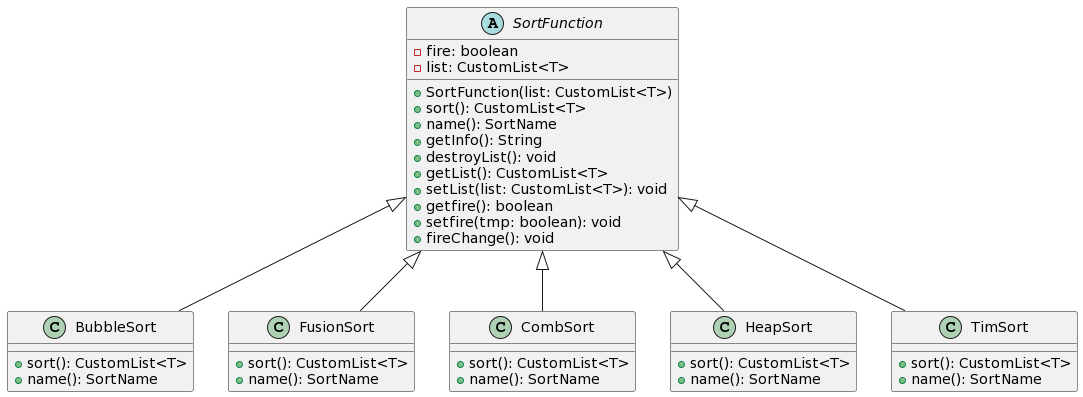
\includegraphics[width=1\textwidth]{sortFunction_UML.png}
    \caption{SortFunction}
    \label{fig:sortFunction}
\end{figure}
\newpage
 Dans le but de faciliter la maintenance et la gestion des algorithmes, nous avons créé une énumération appelée \texttt{SortName}. Cette énumération associe un nom unique à chaque algorithme de tri que nous avons développé.
Par exemple, nous avons inclus des noms tels que \texttt{BubbleSort}, \texttt{QuickSort}, \texttt{InsertionSort}, etc., correspondant à chaque algorithme de tri respectif. De plus, cette énumération est utilisée dans diverses parties de notre code pour des opérations telles que la vue ou pour la collecte de statistiques sur les performances des différents algorithmes.

\begin{figure}[h]
    \centering
    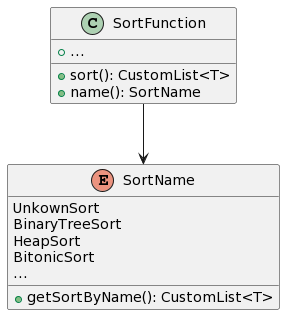
\includegraphics[height=0.5\textwidth]{SortName_UML.png}
    \caption{SortName}
    \label{fig:sortName}
\end{figure}

\subsubsection{Structures de données :}
   
\begin{enumerate}[label=\textbf{\arabic*.} , font=\bfseries]
  

\item \textbf{HeapSort}

L'algorithme HeapSort repose sur l'utilisation d'une structure de données appelée un tas binaire. Un tas binaire est une structure d'arbre binaire où chaque nœud a une valeur qui est plus grande que les valeurs de ses nœuds enfants (pour un tas binaire min) ou plus petite (pour un tas binaire max).

La structure de données de tas binaire a été implémentée dans notre projet en utilisant la classe \texttt{Heap}. Cette classe comporte les caractéristiques suivantes :

\begin{itemize}
    \item \textbf{Liste représentant le tas binaire :} La structure principale du tas binaire est une liste, représentée par l'attribut \texttt{heapArray} de type \texttt{CustomList}. Cette liste contient les éléments du tas binaire.
    \item \textbf{Taille maximale et actuelle :} Le tas binaire a une taille maximale, représentée par l'attribut \texttt{maxSize}, ainsi qu'une taille actuelle, représentée par l'attribut \texttt{currentSize}.
    \item \textbf{Opérations de base :} La classe \texttt{Heap} propose des opérations telles que l'insertion d'un nouvel élément, la suppression du premier élément, la construction du tas à partir d'une liste donnée, et le tri du tas binaire.
\end{itemize}

\begin{figure}[H]
    \centering
    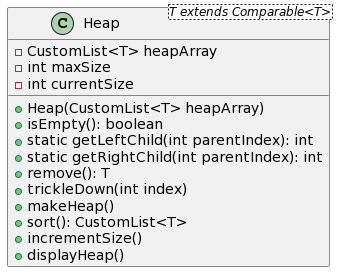
\includegraphics[width=0.5\textwidth]{Heap.png}
    \caption{HEAP}
    \label{fig:heap}
\end{figure}

\item \textbf{Arbre binaire}

L'algorithme HeapSort utilise également une structure de données appelée arbre binaire. Dans notre implémentation, nous avons utilisé la classe \texttt{BinaryTree} pour représenter un arbre binaire. Voici ses caractéristiques :

\begin{itemize}
    \item \textbf{Racine de l'arbre :} La classe \texttt{BinaryTree} comporte un attribut \texttt{root} qui représente la racine de l'arbre binaire.
    \item \textbf{Liste triée :} Lorsqu'un arbre binaire est construit à partir d'une liste donnée, la classe \texttt{BinaryTree} remplit également une liste triée avec les éléments de l'arbre, stockée dans l'attribut \texttt{sorted}.
\end{itemize}

\begin{figure}[H]
    \centering
    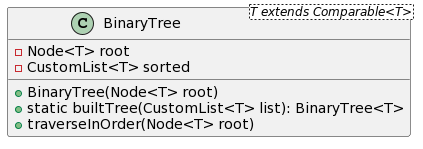
\includegraphics[width=0.5\textwidth]{BinaryTree.png}
    \caption{BinaryTree}
    \label{fig:BinaryTree}
\end{figure}

\item \textbf{Nœud d'arbre binaire}

Chaque nœud dans un arbre binaire est représenté par la classe \texttt{Node}. Voici ses caractéristiques :

\begin{itemize}
    \item \textbf{Valeur du nœud :} Chaque nœud contient une valeur de type générique \texttt{T}.
    \item \textbf{Fils gauche et fils droit :} Un nœud peut avoir un fils gauche et un fils droit, représentés par les attributs \texttt{left} et \texttt{right}.
    \item \textbf{Opérations de base :} La classe \texttt{Node} comporte des méthodes pour vérifier si un nœud a un fils gauche ou un fils droit, ainsi que des méthodes pour comparer les valeurs de deux nœuds et pour insérer un nouveau nœud dans l'arbre.
\end{itemize}

Ces structures de données sont essentielles pour l'implémentation et le fonctionnement de l'algorithme HeapSort dans notre projet. Elles offrent une organisation efficace et une manipulation pratique des données pendant le processus de tri.
\begin{figure}[h]
    \centering
    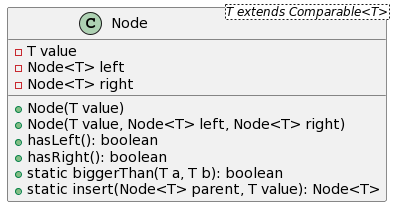
\includegraphics[width=0.5\textwidth]{Node.png}
    \caption{Node}
    \label{fig:mon_image}
\end{figure}
\end{enumerate}
\subsubsection{Médiateur pour la Création d'Algorithmes de Tri}

La classe médiateur, implémentée sous le nom de \texttt{SortCreatorMediator}, joue un rôle crucial dans la facilitation de la création d'instances d'algorithmes de tri dans notre projet. Elle agit comme une interface centrale pour créer des instances de \texttt{SortFunction} en fonction du nom spécifié de l'algorithme de tri et de la liste à trier.\\

\textbf{Classe Médiateur}\\

La classe \texttt{SortCreatorMediator} utilise une approche basée sur le nom de l'algorithme pour instancier les différentes classes d'algorithmes de tri. Elle vérifie le nom fourni et crée une instance appropriée de l'algorithme de tri correspondant.

\begin{itemize}
\item \textbf{Rôle :} La classe médiateur simplifie le processus de création d'instances d'algorithmes de tri en encapsulant la logique de création.
\item \textbf{Interface :} Elle implémente l'interface \texttt{Mediator}, qui définit une méthode \texttt{create} permettant de créer une instance de \texttt{SortFunction}.
\item \textbf{Méthode \texttt{create} :} Cette méthode prend en paramètre le nom de l'algorithme de tri et la liste à trier, et renvoie une instance appropriée de \texttt{SortFunction} correspondante.\\
\end{itemize}
\textbf{Fonctionnement de la Classe Médiateur}\\

La classe \texttt{SortCreatorMediator} utilise une approche basée sur le nom de l'algorithme pour instancier les différentes classes d'algorithmes de tri. Elle vérifie le nom fourni et crée une instance appropriée de l'algorithme de tri correspondant. Par exemple, si le nom est \texttt{SortName.HeapSort}, elle instancie un objet \texttt{HeapSort} avec la liste fournie.

Cette approche simplifie considérablement le processus de création d'instances d'algorithmes de tri en encapsulant la logique de création dans une seule classe. Au lieu d'avoir un code répétitif pour chaque algorithme de tri, nous utilisons cette classe médiateur pour déléguer la responsabilité de création d'instances aux classes d'algorithmes de tri respectives. Cela rend notre code plus modulaire, maintenable et extensible.

La classe médiateur ajoute une couche d'abstraction qui permet de changer facilement les implémentations d'algorithmes de tri sans modifier le code client, ce qui améliore la flexibilité et la maintenabilité de notre projet.\\


\begin{figure}[h]
    \centering
    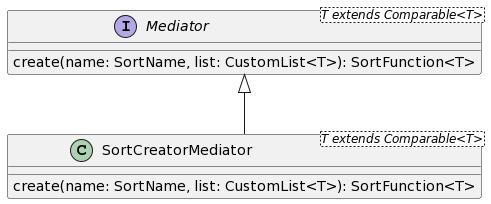
\includegraphics[width=0.5\textwidth]{Mediator.png}
    \caption{Mediator}
    \label{fig:mon_image}
\end{figure}


\section{Générateurs de désordre}
\subsection{Fonctionnement}
Les générateurs de désordre représentent une partie importante de l'analyse des algorithmes. L'objectif est d'appliquer un désordre maîtrisé sur la liste qui sera envoyée à l'algorithme de tri, permettant une analyse plus poussée de celui-ci en le mettant sous différentes contraintes. En effet, un algorithme peut être extrêmement efficace sur un certain type de liste, mais pour autant être l'un des plus lent sur un autre type. Dans cette partie, on ne parle pas de taille de liste, mais bien de type de liste, c'est pourquoi les calculs prenant en compte les désordre sont tous effectués sur une taille de liste fixe.

Cette partie du code est celle qui sera exécuté en premier lors des calculs. Elle se charge de créer une liste triée (ici d'entiers) et de l'enregistrer dans l'instance de CustomList (instanciée dans le contrôleur). Ensuite elle se charge de désordonner la liste de l'instance de CustomList.

Chaque classe de générateur étend une classe abstraite \texttt{Generator}. Elle définit le contrat pour les générateurs. On y retrouve les méthodes \texttt{getName} et \texttt{DisorderAlgorithm}.
\vspace{1cm}
\begin{figure}[h]
    \centering
    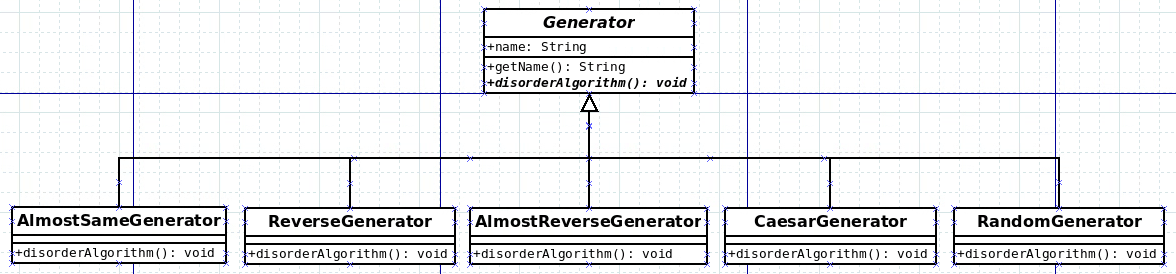
\includegraphics[width=0.9\textwidth]{uml_generator.png}
    \caption{UML de l'héritage des générateurs}
    \label{UML generator}
\end{figure}

\newpage
\subsection{Différents désordres}
Comme mentionné précédemment, ces générateurs créent un désordre maîtrisés (À part RandomGenerator évidemment) sur une liste triée. Leurs noms sont très évocateurs, mais voici leur fonctionnement détaillé :
\vspace{0.5cm}

\begin{enumerate}
    \item \texttt{AlmostSameGenerator} ne va faire qu'échanger la place de deux éléments dans la liste. Ce désordre est ridiculement simple à trier pour un humain, et pourtant, on voit que le temps d'exécution des algorithmes ne sont pas pour autant plus rapides. Ils est même plus long pour certain que pour trier une liste random.
    \item \texttt{ReverseGenerator} permet de renverser les éléments dans la liste. C'est la même chose ici, cet exercice est anodin pour un humain, mais représente une vraie épreuve pour certains algorithmes. 
    \item \texttt{AlmostReverseGenerator} est un mélange des deux générateurs de désordre précédents. Il applique un renversement puis échange deux éléments.
    \item \texttt{CaesarGenerator} est basé sur la méthode de chiffrement à décalage, souvent appelé "code César". Tous les éléments de la liste sont décalés de 1 vers la droite, et le dernier élément vient se placer en première position. On observe une énorme hausse du temps d'exécution pour la plupart des algorithmes avec ce désordre \ref{screenBetter}.
    \item \texttt{RandomGenerator} est le désordre le plus évident. Il mélange aléatoirement les éléments de la liste.
\end{enumerate}
\vspace{1.5cm}
\begin{figure}[h]
\begin{tikzpicture}[node distance=0.8cm]
        %Listes d'origine   
      \node (Liste1) at (-6,0) {(0,1,2,3,4)};

      %Générateur
      \node (Générateur) at (-2,0) {GeneratorFactory};

      %Listes désordonnées
      \node (Liste2) at (4,3) {AlmostSame : 0,1,3,2,4};
      \node (Liste3) at (4,1.5) {Reverse : 4,3,2,1,0};
      \node (Liste4) at (4,0) {AlmostReverse : 4,1,2,3,0};
      \node (Liste5) at (4,-1.5) {Caesar : 1,2,3,4,0};
      \node (Liste6) at (4,-3) {Random : 4,1,2,3,0};

      %Objet CustomList
      \node (CustomList) at (10,0) {CustomList};

      %Flèches
      \draw[->] (Liste1) -- (Générateur);

      \draw[->] (-0.5,0.5) -- (1.8,2.8);
      \draw[->] (-0.3,0.3) -- (2.2,1.5);
      \draw[->] (Générateur) -- (Liste4);
      \draw[->] (-0.3,-0.3) -- (2.3,-1.4);
      \draw[->] (-0.5,-0.5) -- (2.1,-2.8);

      \draw[->] (6.3,2.8) -- (9,0.5);
      \draw[->] (5.8,1.5) -- (8.8,0.3);
      \draw[->] (Liste4) -- (CustomList);
      \draw[->] (5.8,-1.4) -- (8.8,-0.3);
      \draw[->] (6,-2.8) -- (9,-0.5);
\end{tikzpicture}
\vspace{1cm}
\caption{Génération du désordre sur la liste}
\end{figure}
\newpage
\subsection{Premières observations}

Il est naturel de supposer que les algorithmes prendront plus de temps à trier une liste aléatoire, étant donné que c'est dans cette configuration que les humains rencontrent le plus de difficultés. Cependant, l'analyse du graphique présenté révèle que les listes désordonnées traitées par "ReverseGenerator" obtiennent en général le pire résultat pour l'ensemble des algorithmes.

\begin{figure}[h]
    \centering
    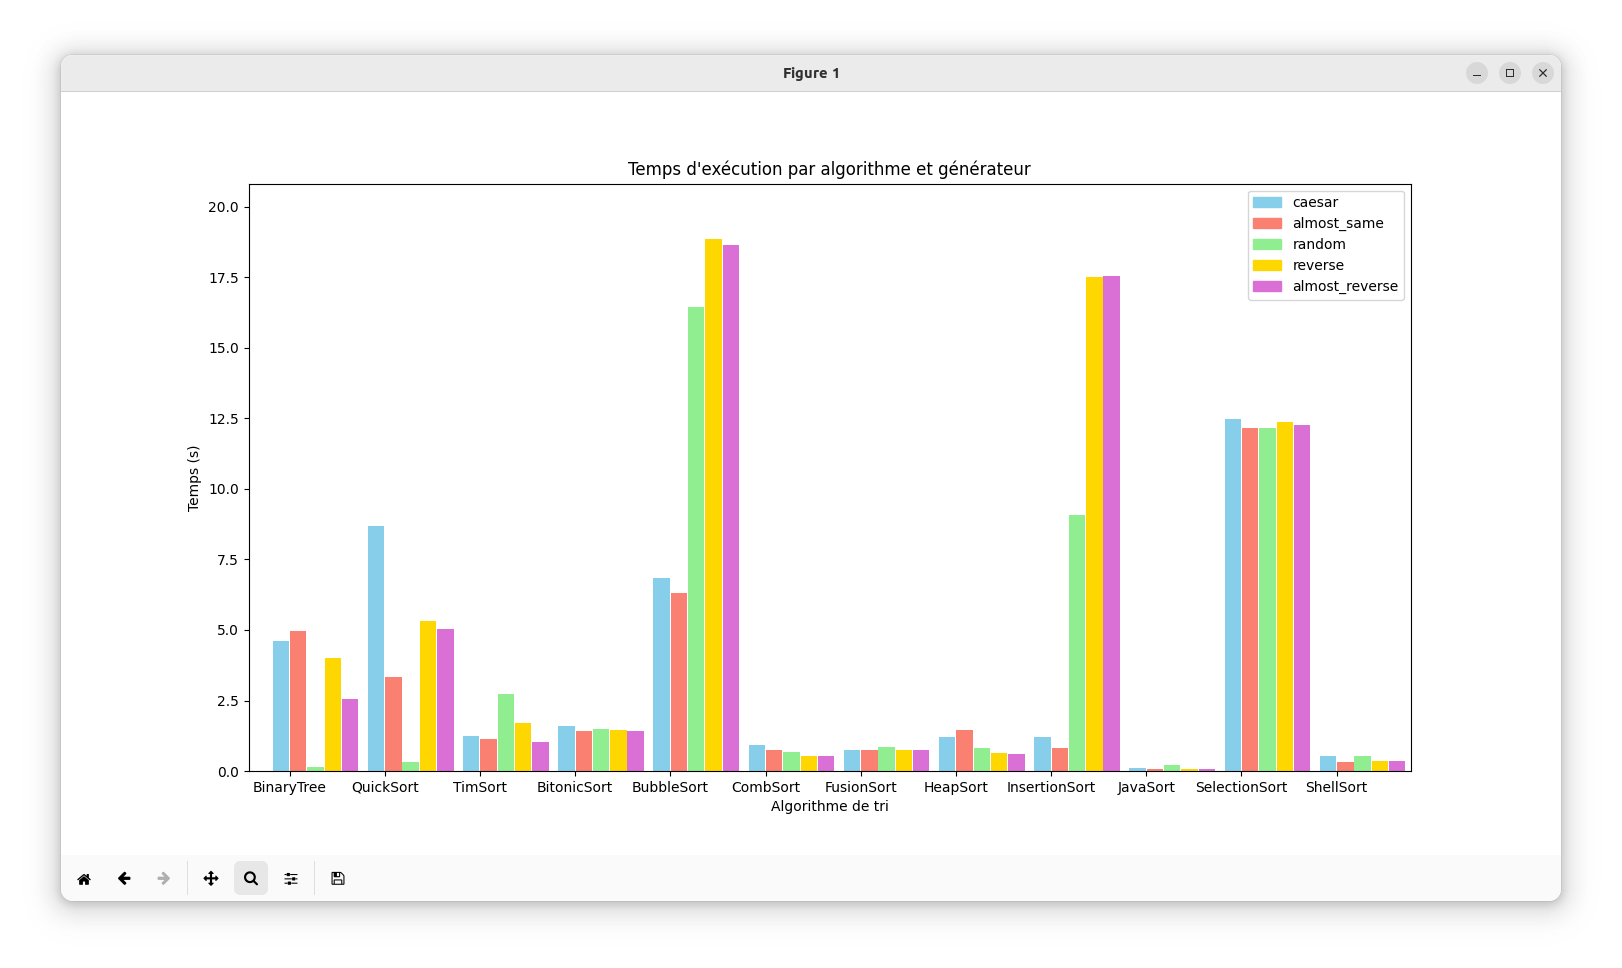
\includegraphics[width=\textwidth]{ScreenBetter.png}
    \caption{Comparaison des temps des algorithmes}
    \label{screenBetter}
\end{figure}

On voit que les algorithmes "BubbleSort", "InsertionSort" et "SelectionSort" sont loin d'être considérés comme rapides quand on les compare aux autres (Sur la taille de liste fixe : 1024).

Aussi, on aperçoit que l'algorithme "QuickSort" est extrêmement efficace sur une liste désordonné de manière aléatoire, à l'inverse sur un désordre "Caesar" il est très lent.

\section{Visualisation des algorithmes}
Pour la visualisation des algorithmes nous nous sommes inspirés de la vidéo fourni dans le sujet : \href{https://www.youtube.com/watch?v=kPRA0W1kECg}{Sound of Sorting}. 
\begin{figure}[h]
    \centering
    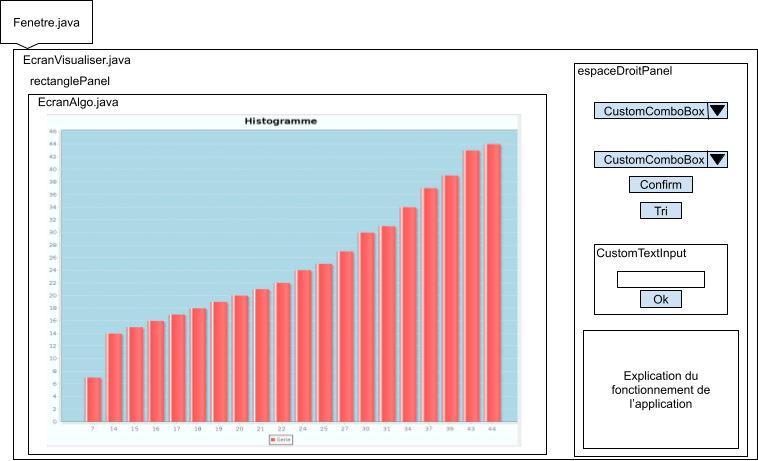
\includegraphics[width=\textwidth]{umlview.png}
    \caption{Wireframe de la vue }
    \label{fig:enter-label}
\end{figure}
\newline
La vue est instanciée par la classe "Fenetre.java". Cette dernière lancera directement la classe "EcranVisualiser.java". Au départ, nous avions envisagé de créer un menu de démarrage, mais nous avons réalisé que cette architecture était plus logique. 
\vspace{0.5cm}
\newline
Au sein de la classe "EcranVisualiser.java", la disposition des composants est divisée en deux parties. Nous avons un panneau principal nommé "rectanglePanel" qui contiendra la visualisation de la liste. Toutes les informations complémentaires et options seront disposées dans le second panneau nommé "espaceDroitPanel".

La visualisation de la liste est réalisé grâce à la librairie JFreeChart. Cette dernière permet de créer un histogramme à partir d'un dataset donné. 

Concernant le second panneau, nous pouvons également le diviser en deux parties. Le premier panneau servira de conteneur pour tous les composants permettant de modifier les options d'affichage. Nous avons créé un composant personnalisé nommé "CustomComboBox", qui hérite du composant "JComboBox<String>". Ce menu déroulant affiche une liste d'options de type "String". De plus, la gestion de la taille de ce composant est effectuée directement dans son propre fichier. Ainsi l'utilisateur peut modifier le générateur de désordre à appliquer sur la liste et l'algorithme qui triera la liste. Le second composant personnalisé "CustomTextInput" est légérement plus complexe. Il permet en effet à l'utilisateur de changer la taille de la liste. Le texte donné en entrée va être vérifié grâce a à la fonction "Integer.parseInt()". Si le texte est un entier et qu'il est supérieur à 0 alors le composant notifie le contrôleur qu'il doit changer la taille de la liste. Sinon un message d'erreur est renvoyé au parent qui va se charger de l'afficher. Enfin en bas du second panneau est expliqué le fonction de l'application. C'est également à ce niveau que certaines remarque sont mises comme par exemple que le "BitonicSort" nécessite une liste dont la taille est une puissance de 2 afin de fonctionner. 
\section{Expérimentation}
Le but de la partie expérimentale est de répondre à notre problématique en suivant une démarche scientifique. Afin de donner un résultat le plus fiable voici la démarche que nous avons suivi : 
    \begin{itemize}
        \item Définition des conditions expérimentales : Cela inclut la taille de la liste, le choix de l'algorithme de tri, ainsi que le niveau de désordre initial de la liste.
        \item Répétition des expériences : Nous avons répété chaque expérience en veillant à reproduire scrupuleusement les mêmes conditions à chaque itération.
        \item Comparaison des résultats : Une fois les expériences menées, nous avons analysé et comparé les résultats obtenus afin d'extraire des conclusions significatives."
    \end{itemize}
\subsection{Réalisation de la partie expérimentale}
Afin de réaliser la partie expérimentale nous avons défini des Writers et des Readers. Le premier s'occupe de définir les conditions expérimentales et de répéter l'expérience, ensuite il écrit les résultat dans un fichier csv. Le second va récupérer le contenu des fichiers csv afin de les rendre visuellement dans le but d'interpréter et de comparer les résultats.\\


Nous avons mené deux analyses distinctes. La première, plus générale, se concentre sur les temps d'exécution pour une même taille de liste. Ainsi, nous pouvons comparer les algorithmes entre eux et les évaluer sur chaque générateur de désordre. Dans la seconde analyse, nous nous sommes penchés sur un algorithme spécifique, en variant la taille de la liste pour observer la sensibilité de cet algorithme à la taille des données traitées.

\subsubsection{Mesure du Temps d'Exécution des Algorithmes de Tri}

La classe \texttt{TimeDecorator} a été conçue pour mesurer le temps d'exécution des différents algorithmes de tri implémentés dans notre projet. Elle agit comme un décorateur qui enveloppe un algorithme de tri spécifique et mesure le temps nécessaire pour trier une liste donnée.\\



La classe prend en charge les fonctionnalités suivantes :

\begin{itemize}
    \item \textbf{Initialisation :} Lors de l'instanciation, elle prend un objet de type \texttt{SortFunction} en paramètre, qui représente l'algorithme de tri à mesurer.
    \item \textbf{Mesure du Temps :} La méthode \texttt{measureTime()} est responsable de mesurer le temps d'exécution de l'algorithme de tri. Elle enregistre également des informations pertinentes telles que le nom de l'algorithme, la taille de la liste à trier et le temps d'exécution formaté.
    \item \textbf{Test :} La méthode statique \texttt{test()} est fournie pour tester le fonctionnement du \texttt{TimeDecorator} avec un algorithme de tri spécifique.
    \item \textbf{Calcul de la Moyenne :} La méthode statique \texttt{averageTimeExecution()} permet de calculer le temps d'exécution moyen de l'algorithme en effectuant plusieurs mesures et en calculant la moyenne.\\
\end{itemize}
Pour utiliser la classe \texttt{TimeDecorator}, il suffit de créer une instance avec un algorithme de tri spécifique, d'appeler la méthode \texttt{measureTime()} pour mesurer le temps d'exécution, et enfin d'accéder aux informations enregistrées via les méthodes d'accès appropriées.
\begin{figure}[h]
    \centering
    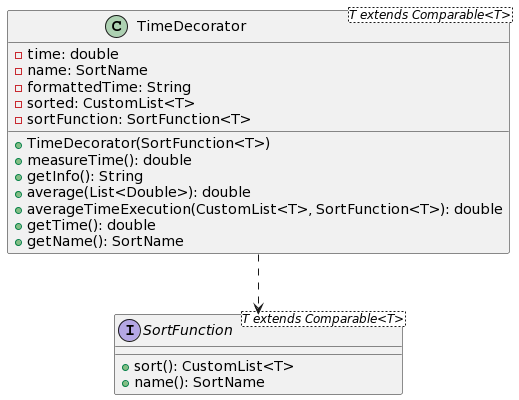
\includegraphics[width=0.45\textwidth]{TimeDecorator.png}
    \caption{TimeDecorator}
    \label{fig:mon_image}
\end{figure}

\subsection{Analyse générale des temps d'exécution}
Notre problématique étant de comparer les algorithmes nous avons réalisés cette comparaison générale. Le but est de tester l'ensemble des algorithmes sur l'ensemble des générateurs afin de définir dans quels conditions chaque algorithme performe le mieux en temps. 
\begin{figure}[H]
  \centering
  \begin{minipage}[b]{0.45\textwidth}
    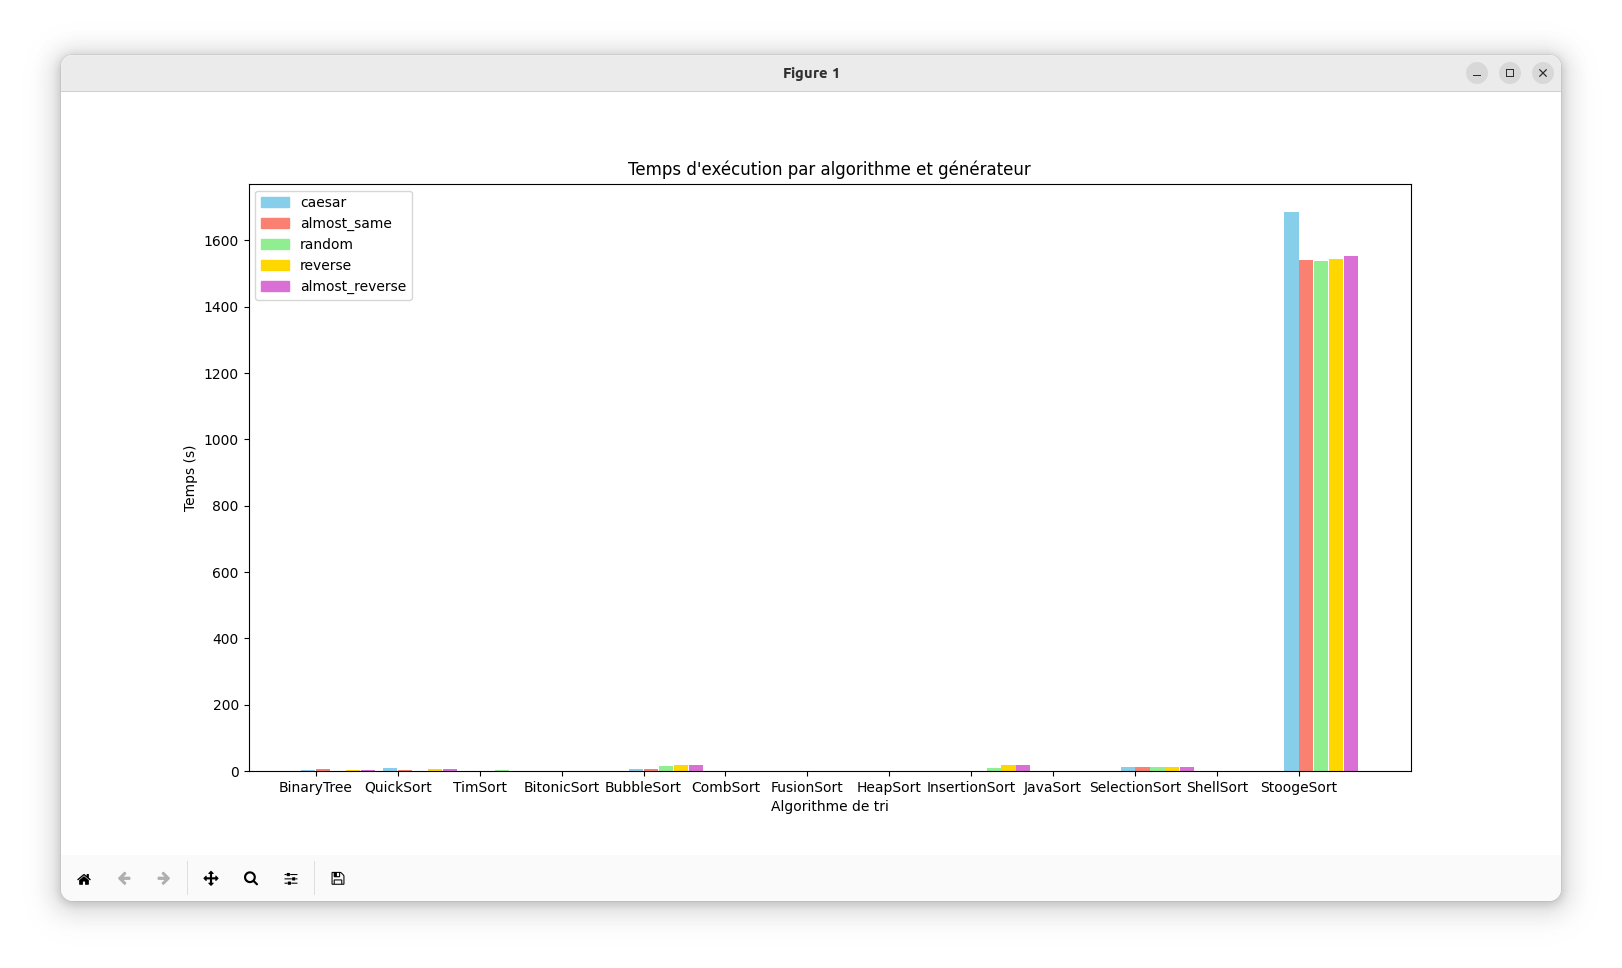
\includegraphics[width=\textwidth]{ScreenWithStooge.png}
    \caption{Comparaison des temps des algorithmes}
    \label{fig:ScreenWithStooge}
  \end{minipage}
  \hfill
  \begin{minipage}[b]{0.45\textwidth}
    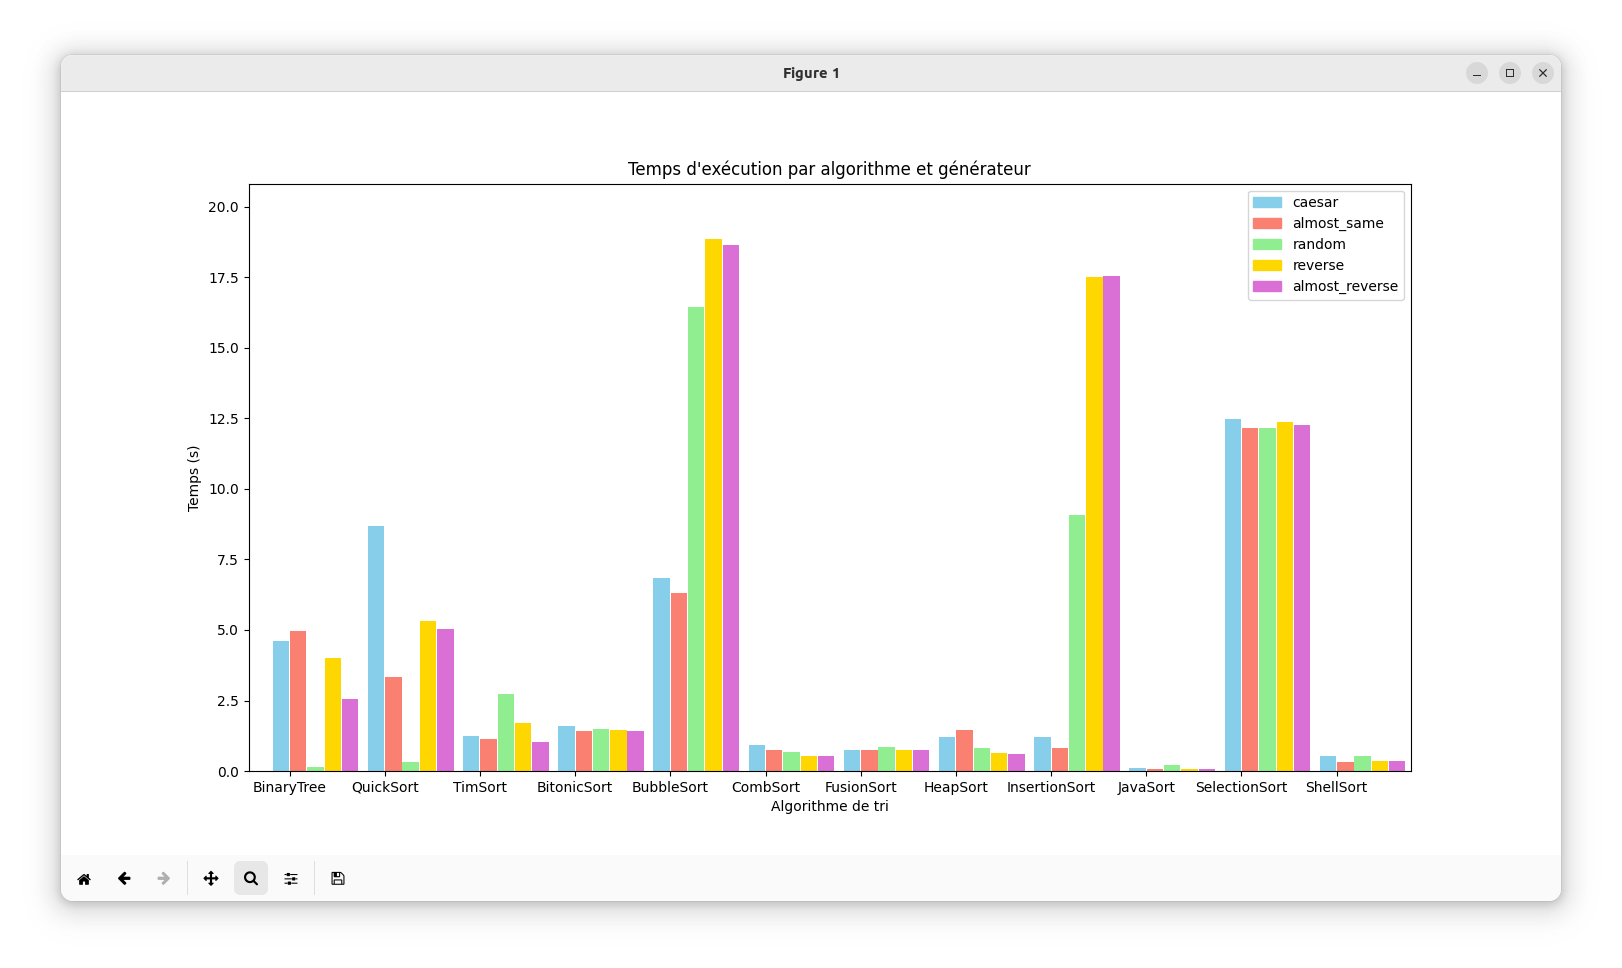
\includegraphics[width=\textwidth]{ScreenBetter.png}
    \caption{Comparaison sans "StoogeSort"}
    \label{fig:ScreenBetter}
  \end{minipage}
\end{figure}
À partir de ces résultats, plusieurs constats évidents peuvent être faits. Premièrement, il est clair que le tri Stooge est très peu performant en termes de temps, sa complexité en temps de $n^{2.71}$
rends l'interprétation des résultats plus difficile. Une fois que "StoogeSort" est écarté, la comparaison entre les algorithmes devient plus simple. 

Ainsi, nous pouvons constater que la majorité des algorithmes sont peu efficaces sur le générateur de désordre "Reverse" et aussi "Almost\_reverse" du à la proximité de ces deux générateurs.

On voit que le "ShellSort" est l'algorithme implémenté le plus constant, indépendamment du type de désordre, et "JavaSort" montre des temps d'exécution record.

\vspace{0.5cm}
Par soucis de clarté, nous ne préciserons plus que ces résultats sont obtenus sur des listes de taille 1024 et nous estimons les résultats obtenus corrects.
\newline
Parmi tous les algorithmes testés lors de cette étude, nous pouvons les répertorier en 3 grandes classes :
\begin{itemize}
    \item \texttt{Les algorithmes "lents"} : StoogeSort, BubbleSort, SelectionSort et InsertionSort sont les algorithmes de loin les plus lents. On compte pour ces algorithmes un temps moyen de 1.5sec, sauf "Stooge Sort" qui met environ 150sec soit 2min et 30 sec. À noter que BubbleSort et InsertionSort sont tous les deux très sensibles au désordre. Si les deux sont relativements lents dans l'ensemble, les résultats sur le désordre "Caesar" et "Almost\_Same" sont jusqu'à 7 fois plus rapide pour le tri par insertion.  
    \item \texttt{Les algorithmes "corrects"} : BinaryTree, QuickSort, TimSort, BitonicSort, HeapSort et ShellSort. Ces algorithmes sont pour la plupart très efficace sur la plupart des listes, mais sont handicapés par leur lenteur sur les listes de type "Caesar". Cette classe d'algorithme à un temps d'exécution moyen de 0,2sec.
    \item \texttt{Les algorithmes "Très efficaces"} : ComboSort, ShellSort, FusionSort et JavaSort. Ils sont les algorithmes les plus rapide, et de loin. Ces deux algorithmes ont un temps d'exécution inférieur à  0.01sec. À noter que le tri Heap ou Insertion pourrait rentrer dans cette catégorie en fonction du désordre. 
    \end{itemize}
    
    Il est remarquable de constater que JavaSort affiche de loin le temps d'exécution moyen le plus rapide. Cette performance s'explique par le fait que JavaSort est un algorithme hybride, combinant différentes philosophies algorithmiques pour obtenir les meilleurs résultats.
    
    Par ailleurs, il est pertinent de souligner que les algorithmes classés comme "corrects" démontrent une efficacité notable dans la plupart des cas. Cependant, le désordre "Caesar" entraîne des temps d'exécution plus longs pour les algorithmes de cette catégorie. Un exemple frappant est celui du "QuickSort" : tandis que sur une liste aléatoire il affiche un temps d'exécution d'environ 0.03s, sur un désordre "Caesar" on peut observer des temps pouvant atteindre 0.8s.
        
    Enfin, les temps d'accès aux différents types de données peuvent avoir un impact significatif sur le choix de l'algorithme. Bien que nos tests aient été réalisés sur des listes de 1024 éléments, il est important de reconnaître que les performances des algorithmes peuvent varier selon la taille des données. Par conséquent le choix d'un algorithme de tri ne doit donc pas se faire seulement en fonction de la comparaison des temps d'exécution. En effet, pour obtenir les meilleurs résultats, il est impératif de définir soigneusement les conditions dans lesquelles le tri sera effectué. Ainsi, en prenant en compte la taille de la liste à trier, le type de structure de données et le niveau de désordre appliqué, nous pouvons effectuer un choix plus adapté à notre situation.
\subsection{Analyse approfondie}
\subsubsection{Démonstration de la Complexité de l'Algorithme de Tri}
Pour démontrer la complexité d'un algorithme de tri, nous avons mené une série d'expériences en mesurant le temps d'exécution de l'algorithme sur des listes de différentes tailles. Les données réelles obtenues ont ensuite été utilisées pour tracer une courbe représentant la relation entre la taille de la liste et le temps d'exécution de l'algorithme.\\

\textbf{Collecte des Données}

Nous avons exécuté l'algorithme de tri sur des listes de différentes tailles, enregistrant le temps d'exécution à chaque itération. Cette opération a été répétée pour plusieurs tailles de listes afin de collecter des données significatives. Les tailles de listes ont été choisies de manière à couvrir une plage significative, allant des petites listes aux grandes.\\

\textbf{Analyse des Données}

Après la collecte des données, nous avons procédé à une analyse pour évaluer les performances de l'algorithme de tri sur des données réelles. Tout d'abord, nous avons récupéré les données à partir d'un fichier CSV contenant des informations sur le temps d'exécution de l'algorithme pour différentes tailles de listes.

Ensuite, nous avons utilisé un script Python nommé \texttt{reader.py} pour lire et traiter ces données. Ce script a fait appel aux bibliothèques Python telles que Matplotlib, Pandas et NumPy pour la manipulation et la visualisation des données.

Plus précisément, nous avons utilisé Pandas pour lire les données à partir du fichier CSV et NumPy pour effectuer des opérations numériques sur ces données. Ensuite, à l'aide de Matplotlib, nous avons tracé la courbe du temps d'exécution en fonction de la taille de la liste.

Cette analyse nous a permis d'obtenir une représentation visuelle du comportement de l'algorithme sur des données réelles, ce qui nous a aidés à évaluer sa performance et à comparer les résultats avec les prévisions théoriques.
\\

\textbf{Comparaison avec la Complexité Théorique}

En comparant la courbe empirique avec la courbe théorique de complexité de l'algorithme, nous pouvons tirer des conclusions sur l'efficacité de l'algorithme. Nous vérifions si son comportement correspond à ce qui est attendu en termes de complexité temporelle. Cette analyse comparative nous permet de valider empiriquement la complexité de l'algorithme de tri et d'évaluer sa performance dans des conditions réelles d'utilisation.\\

\textbf{Interprétation des Résultats}

Les résultats obtenus fournissent des informations précieuses sur le comportement réel de l'algorithme de tri en fonction de la taille des données. En comparant la courbe empirique du temps d'exécution avec la courbe théorique, nous pouvons observer si l'algorithme se comporte conformément à nos attentes.

Nous constatons que les données obtenues suivent de près la courbe théorique, ce qui indique une cohérence entre les performances attendues et observées de l'algorithme. Cette concordance renforce notre confiance dans l'efficacité de l'algorithme dans des scénarios réels.\\
\subsubsection{Analyse de la Complexité des Algorithmes de Tri}
Dans cette section, nous avons réalisé une étude approfondie de la complexité des algorithmes de tri en utilisant des données générées à partir de différentes tailles de listes et de différents types de listes. Plus spécifiquement, nous avons examiné le comportement des algorithmes de tri par rapport à deux types de données : presque inversées et aléatoires.

Les résultats de nos expériences ont révélé des tendances significatives dans le temps d'exécution des algorithmes en fonction de la taille des listes. Pour les algorithmes de complexité quadratique tels que le tri par sélection et le tri par insertion, nous avons observé une croissance quadratique du temps d'exécution en fonction de la taille des listes presque inversées. En revanche, pour les algorithmes de complexité $O(n \log n)$ tels que le tri fusion et le tri rapide, nous avons constaté des courbes de temps d'exécution de type $kn \log n$ pour des listes de taille variable.

Ces observations confirment les propriétés attendues des algorithmes de tri en fonction de leur complexité. Les courbes de temps d'exécution obtenues illustrent clairement la différence de comportement entre les algorithmes de complexité quadratique et ceux de complexité $O(n \log n)$. Cette analyse de la complexité nous permet de mieux comprendre les performances des algorithmes de tri dans des scénarios réels et de prendre des décisions éclairées lors du choix de l'algorithme le plus approprié pour une application donnée. \\

\textbf{Test de l'algorithme de tri}\\


Pour évaluer les performances des algorithmes de tri, nous avons effectué une série de tests sur des listes de différentes tailles. À cet effet, nous avons généré des listes d'entiers variant de 1000 à 100000 éléments à l'aide d'un générateur presque inversé. Ce générateur produit des listes dans lesquelles les éléments sont quasiment dans un ordre décroissant. Cette approche de génération de données constitue un cas de test pertinent pour évaluer la capacité des algorithmes à traiter des données presque triées.

Après la génération des listes, nous avons appliqué différents algorithmes de tri à chacune d'elles, mesurant ainsi le temps d'exécution requis pour trier les éléments. Par la suite, nous avons représenté graphiquement ces résultats afin de visualiser la relation entre la taille des listes et le temps d'exécution de chaque algorithme.\\ \\
\newpage

Les figures ci-dessous présente les résultats de nos tests avec l'algorithme de tri FusionSort, InsertionSort et BubbleSort. Sur l'axe horizontal, nous observons la taille des listes, tandis que sur l'axe vertical, nous représentons le temps d'exécution en millisecondes.
\begin{figure}[H]
    \centering
    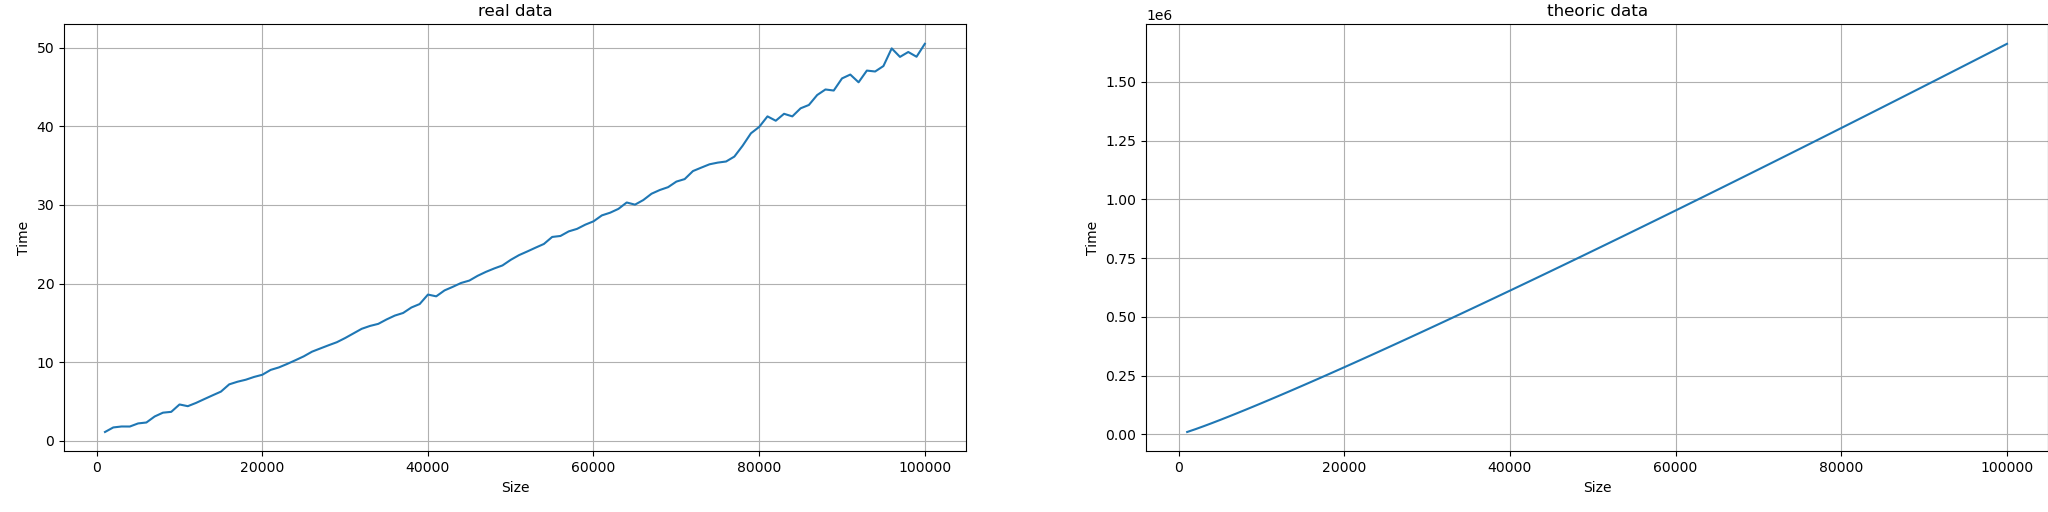
\includegraphics[width=\textwidth]{FusionSort.png}
    \caption{FusionSort}
    \label{fig:mon_image}
\end{figure}


\begin{figure}[H]
    \centering
    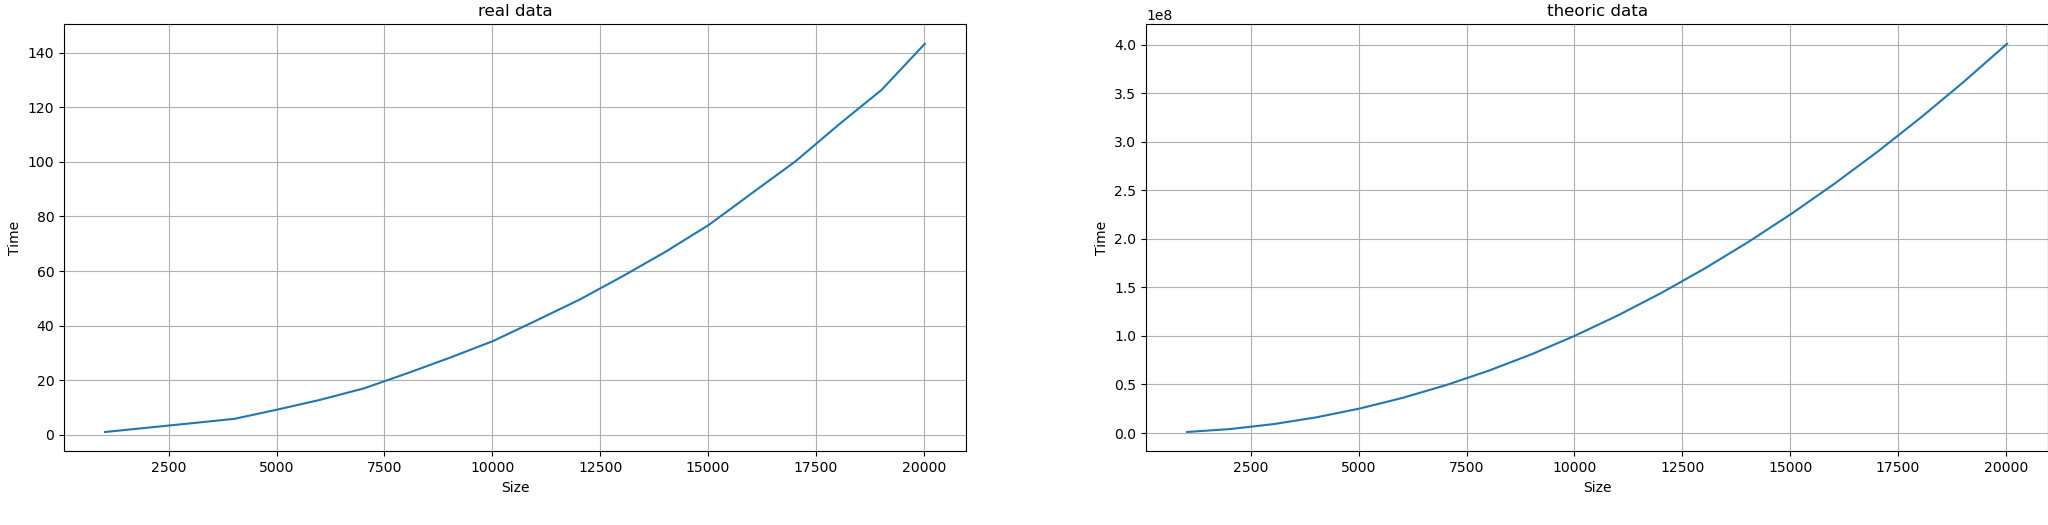
\includegraphics[width=\textwidth]{InsertionSort.png}
    \caption{InsertionSort}
    \label{fig:mon_image}
\end{figure}

\begin{figure}[H]
    \centering
    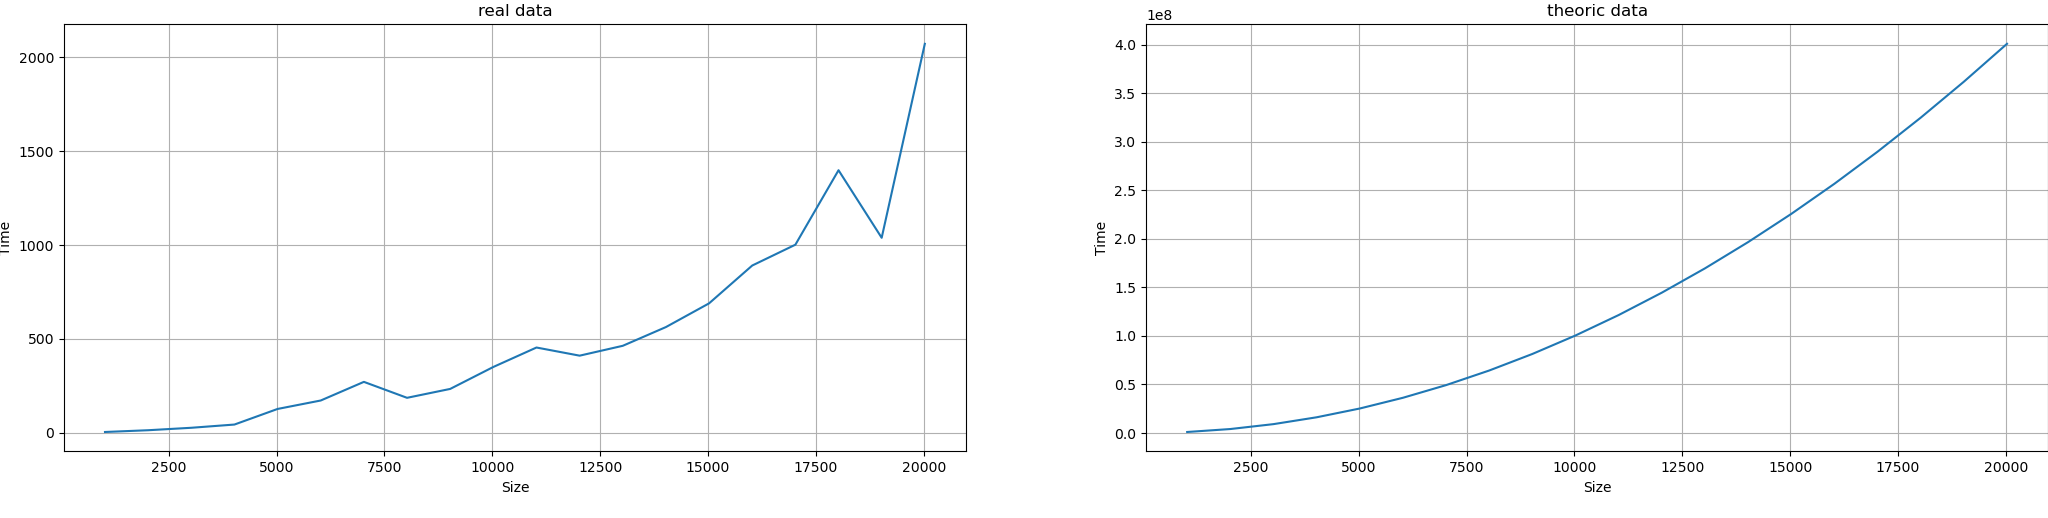
\includegraphics[width=\textwidth]{BubbleSort.png}
    \caption{BubbleSort}
    \label{fig:mon_image}
\end{figure}
\newpage
\subsection{Autres analyses}
    Nous avons également pu comparer le nombre d'accès à la liste ainsi que le nombre de comparaison effectués à l'aide du \textit{décorateur} "TimeDecorator". Les résultats suivants ont été obtenus en exécutant l'ensemble des algorithmes sur les 5 générateurs puis en effectuant une moyenne du nombre d'accès et de comparaison. 
    
    \begin{table}[htbp]
    \centering
    \begin{tabular}{|l|c|c|}
        \hline
        \textbf{Tri} & \textbf{Nombre d'accès} & \textbf{Nombre de comparaisons} \\
        \hline
        BinaryTreeSort & 2048 & 0 \\
        HeapSort & 64 958 & 38 526 \\
        BitonicSort & 225 280 & 112 640 \\
        ShellSort & 44 027 & 21 830 \\
        TimSort & 52 131 & 28 408 \\
        CombSort & 92 099 & 41 405 \\
        FusionSort & 2048 & 20 480\\
        QuickSort & 56 0246 & 558 416 \\
        InsertionSort & 445 729 & 222 864 \\
        SelectionSort & 2 095 104 & 1 047 552 \\
        BubbleSort & 1 002 665 & 501 332 \\
        StoogeSort & 258 280 324 & 129 140 162 \\
        JavaSort & 0 & 0 \\
        \hline
    \end{tabular}
    \caption{Comparaison des performances des algorithmes de tri}
    \label{tab:sorting_comparison}
    \end{table}
    
    De par son implémentation il est difficile de recueillir des résultat cohérent pour "BinaryTree" nous allons donc l'ignorer par la suite. Il est important de noter que "JavaSort" ne possède pas de résultat nul. Cependant, comme nous n'avons pas accès au code de cet algorithme, nous n'avons pas pu implémenter notre \textit{décorateur}. Toutefois, nous pouvons apprendre dans la documentation
    \footnote{\href{https://docs.oracle.com/javase/8/docs/api/java/util/List.html}{This implementation is a stable, adaptive, iterative mergesort that requires far fewer than n lg(n) comparisons when the input array is partially sorted, while offering the performance of a traditional mergesort when the input array is randomly ordered. If the input array is nearly sorted, the implementation requires approximately n comparisons. Temporary storage requirements vary from a small constant for nearly sorted input arrays to n/2 object references for randomly ordered input arrays.}}
    que le nombre d'accès à la liste pour "JavaSort" est comparable a un "mergeSort". Cependant sa compléxité en espace est variable en terme fonction du type de désordre. 
    
    
    
    Plusieurs observations sont à noter quant à ces résultats. Le tri fusion semble toujours se démarquer, de la même façon que "StoogeSort" obtient les pires résultats. 
\section{Conclusion}
En conclusion, l'algorithme que nous avons implémenté et qui obtient les meilleurs résultats est de loin le "ShellSort". En termes de temps, il est comparable à "JavaSort", qui repose sur un algorithme dit "hybride" combinant différents algorithmes de tri pour obtenir le meilleur résultat. Cependant, comme mentionné précédemment, le choix d'un algorithme de tri ne doit pas se baser uniquement sur des comparaisons numériques. Il est essentiel d'identifier le type de données à traiter, le niveau de désordre et l'ensemble des paramètres d'utilisation. En effet, nous avons observé avec par exemple "HeapSort" obtient une complexité en espace très intéressante grâce à sa structure de données.

Le niveau de désordre influence également fortement le choix de votre algorithme. En nous basant sur le graphique \ref{screenBetter}, il est évident que pour un niveau de désordre aléatoire, "QuickSort" se révèle très efficace. En revanche, pour les autres niveaux de désordre, on privilégiera d'autres algorithme tel que "TimSort". De même, "InsertSort"  peut donner des résultats en temps très intéressants, mais il convient de l'éviter dans le cadre d'un désordre de type "Reverse" ou "Almost\_Reverse".\\


Les résultats de nos tests fournissent également des informations précieuses sur les performances des algorithmes de tri étudiés. Nous avons observé que pour des listes de taille croissante, le temps d'exécution des algorithmes de tri augmente de manière significative. Cette tendance confirme la complexité temporelle des algorithmes de tri, notamment ceux de complexité quadratique comme le tri par insertion et le tri par sélection, et ceux de complexité quasi-linéaire comme le tri fusion et le tri rapide.

\end{document}
